\documentclass[11pt]{article}
\usepackage{amsmath, amssymb}
\usepackage{geometry}
\geometry{margin=1in}
\usepackage{fancyhdr}
\usepackage{lastpage}
\usepackage{parskip} % Better paragraph spacing
\usepackage{titlesec} % Better section formatting
\usepackage{graphicx}
\usepackage{float}
\usepackage[most]{tcolorbox}
\usepackage{lmodern}
\usepackage{caption}
\usepackage{hyperref}

% Define commands for reusable content
\newcommand{\coursename}{COM-402 Information Security and Privacy}
\newcommand{\lecturenum}{09}
\newcommand{\lecturedate}{\today}
\newcommand{\professor}{Mathias Payer}

\hypersetup{colorlinks=true,linkcolor=blue,urlcolor=blue}

% Configure section spacing
\titlespacing*{\section}{0pt}{2ex plus 1ex minus .2ex}{1.5ex plus .2ex}
% Header / Footer
\pagestyle{fancy}
\fancyhf{}
\fancyhead[L]{\coursename}
\fancyhead[R]{Lecture \lecturenum}
\fancyfoot[L]{EPFL - Computer Science}
\fancyfoot[C]{Author: Jonathan Dutoit}
\fancyfoot[R]{Page \thepage\ of \pageref{LastPage}}

\begin{document}

\begin{center}
  {\large EPFL - Computer Science} \\[0.5em]
  {\Large \textbf{\coursename}} \\[0.5em]
  {\large Lecture \lecturenum\ --- \lecturedate} \\[0.5em]
  {\large Author: Jonathan Dutoit} \\[0.5em]
  {\large Professor: \professor} \\[0.5em]
\end{center}

\vspace{2cm}
\begin{center}
  {\LARGE \textbf{Network Security}}
\end{center}

\vspace{1cm}

\section*{Learning goals}

\begin{itemize}
	\item Understand Network request
	\item Learn about Firewalls and Intrusion Detection Systems
	\item Data protection best practices
\end{itemize}

\section*{Outline}

\begin{itemize}
	\item Protecting the Network
	\item Protecting Remote Access
	\item Protecting the Perimeter
		\begin{itemize}
			\item Firewalls and Zones
			\item Firewall rules
			\item Proxies
			\item Intrusion detection systems
		\end{itemize}
	\item Protecting the Workstation
	\item Protecting the Past (logging)
	\item Protecting Data (backups)
\end{itemize}

\section*{Security Breach at Target}

Malware installed in Target's security and payment system, stealing details of every credit card used at the company's 1,797 US stores. 

Security alerts on Dec 2, 2014. Target takes two weeks to react. 

Result: 40 million credit card numbers stolen

The hacker(s) got in by compromising a third-party vendor.

\section*{Network Security Best Practices}

\textbf{\textit{Inside}} the network: segment the network physically:
\begin{itemize}
	\item Different zones for different parts of the organization
	\item Demilitarized zone (DMZ)* to expose organization's external facing network on the internet
\end{itemize}

Towards \textit{\textbf{outside}} secure communication
\begin{itemize}
	\item TLS, IPSec, VPNs
\end{itemize}

\section*{Network (micro) Segmentation}

Break down the network into segments based on system and data classification or into functional zones. Access from zone to zone can be managed by access control lists (ACLs) in routers or firewalls.

Mainly addresses two points:
\begin{itemize}
	\item Prevents all-at-once compromise of facilities
	\item Protects the data center from external threats (little protection against internal threat agents)
\end{itemize}

\section*{Network Segmentation: Rings}

In the classic \textit{concentric architecture} access rights to services increase with each level, moving between levels is managed by access control. 

One single ring may contain diverse services and many machines. An attack spreading in that ring may create significant damage. 

% Quick centered image
\begin{figure}[H]
    \centering
    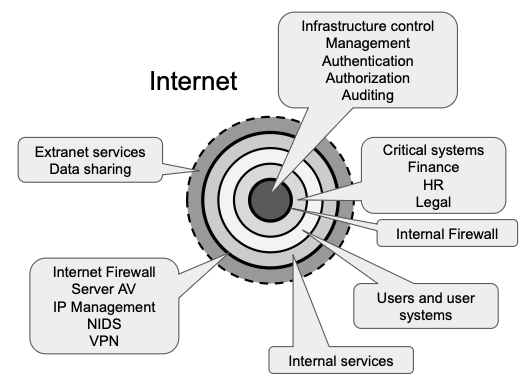
\includegraphics[width=0.6\textwidth]{rings}
    \label{fig:LABEL}
\end{figure}


Advantage: \textbf{less complex}. Disadvantage: \textbf{Shared access between services that are maybe not linked}


\section*{Demilitarized Zone (DMZ)}

A physical or logical subnetwork that contains and exposes an organization's external-facing services to an untrusted network, e.g. Iternet

An external network node can access only what is exposed in the DMZ

The most common services in DMZ are web, email, DNS, and VPN servers

% Quick centered image
\begin{figure}[H]
    \centering
    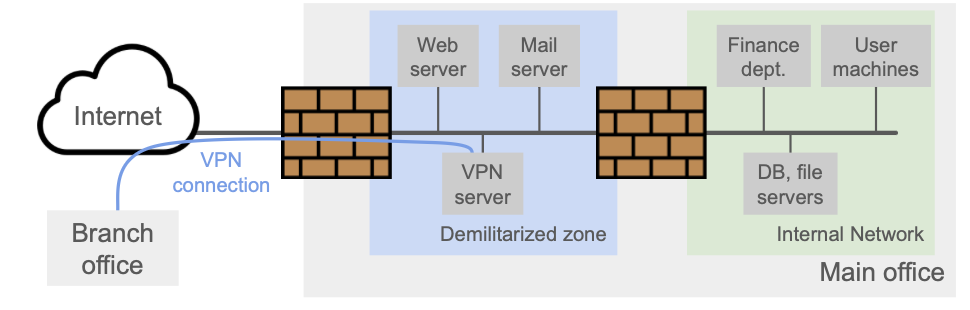
\includegraphics[width=0.8\textwidth]{dmz}
    \label{fig:LABEL}
\end{figure}

There are two possible architectures: \textbf{single} firewall and \textbf{dual} firewall. One is less complex but less secure. The other is more complex and more secure. 

Note that a single configuration mistake is more severe in a single firewall architecture. 

\section*{Network Segmentation: Zones}

Creating containment zones aims to stop attacks from spreading between zones. We want to have real fine-grained zones for a network. 

Communication between zones goes through firewalls. This is closer to \textbf{least privilege} than rings. 

The challenge is creating firewall rules for each case, it's easy to make mistakes and hard to keep rules updated/in sync. 

\section*{Virtual Segmentation}

\begin{tcolorbox}[
  colback=orange!15,     % background color
  colframe=black!50,    % border color
  boxrule=1pt,       % border thickness
  arc=3mm,             % rounded corners
  left=4mm, right=4mm, top=2mm, bottom=2mm % padding
]
How and where would you implement VLAN segmentation?
\end{tcolorbox}

Network zones differ from physical zones, e.g., the HR zone spans two buildings

\textbf{\textit{Virtual LAN}} (VLAN) technology compartmentalizes several layer 2 networks (ethernet) over the same cables and switches, any socket in any building can be configured to belong to any layer 2 network. 

\textbf{\textit{Virtual Routing and Forwarding}} (VRF) allows a single router to be part of several IP networks with VLAN and VRF, any socket in any location can be configured to belong to any ethernet and IP network

\textbf{\textit{Virtual Machines}} (VMS) allows coalescing several servers and routers on a single hardware rack. The web server in the DMZ may actually be running on the same physical machine as the database of the internal back-end zone!

\section*{New Angle: "Zero Trust" Networks}

Do not trust anybody, not even internal machines
\begin{itemize}
	\item Goal: prevent lateral movement
	\item Continuously monitor and validate everything
	\item Install local firewall on internal machines (least privilege and access control)
	\item Encrypt all traffic between internal machines (microsegmentation)
	\item Use strong authentication even internally (MFA)
\end{itemize}

More work to configure machines, but with modern techniques (dockers, kubernetes) configuring and rolling out virtual machines can be automated. 

Less work on configuring the network. Greatly reduces the impact if one machines is compromised. 

\textbf{Note}: security comes at cost, if users have to fill 2FA 15x a day then there's an issue. 

\vspace{0.5cm}

\begin{center}
  {\LARGE \textbf{Protecting Remote Access}} \\
  \vspace{0.2cm}
  Virtual Private Networks
\end{center}
\vspace{0.5cm}

\section*{Virtual Private Networks (VPNs)}

A VPN runs a \textit{\textbf{private, virtual}} network over a \textbf{\textit{public, physical}} network using two key components:
\begin{itemize}
	\item Encryption to keep it private and for confidentiality 
	\item Encapsulation packing IP packets inside IP packets to hide internal addresses and to transport private packets over the public network
\end{itemize}

A distant network or single machines can access a VPN through a VPN gateway

A single machine can run a VPN software to create a virtual interface, this interface has an IP address in the VPN network

Before a packet is sent over the public network, it is encrypted and encapsulated with an IP header with the public addresses.

% Quick centered image
\begin{figure}[H]
    \centering
    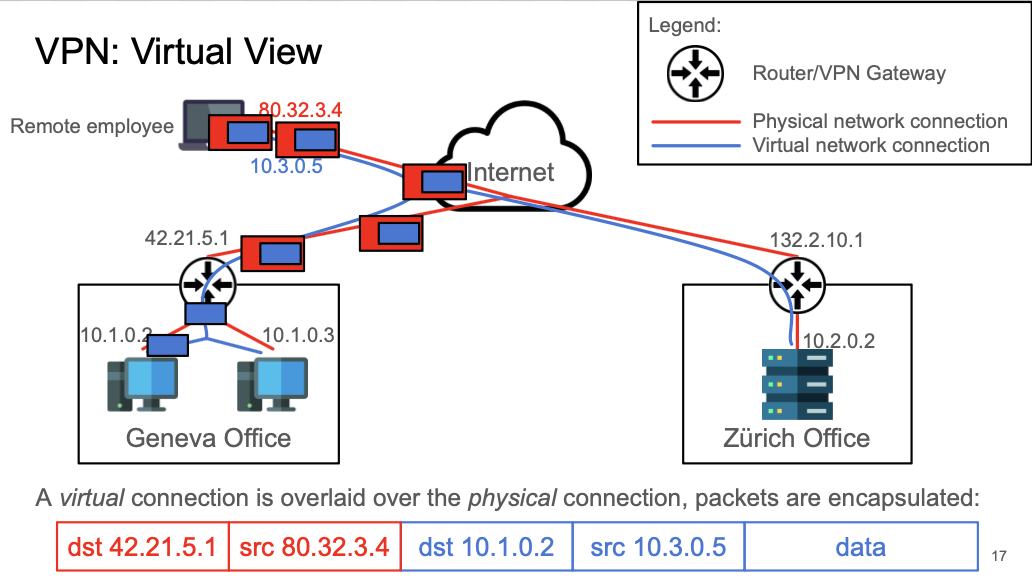
\includegraphics[width=0.8\textwidth]{vpn}
    \label{fig:LABEL}
\end{figure}

\textcolor{red}{Physical network interface} has public IP address and a hardware address, \textcolor{blue}{virtual VPN interface} shows up like just another network interface but \textbf{\textit{without}} hardware address and an IP address from the private space!

\section*{VPN}

\textbf{Typical networks}
\begin{itemize}
	\item IP,sec, official IETF standard
	\item OpenVPN, open source software, based on TLS
	\item WireGuard, built into the Linux Kernel
	\item Proprietary protocols (e.g., Cisco AnyConnect), offer convenience in configuration and maintenance
\end{itemize}

\textbf{Typical use}
\begin{itemize}
	\item Letting remote workers access the internal company network
	\item Interconnecting remote sites of a company
	\item For us: Acessing university resources (e.g, download papers)
	\item For us: Playing CTF and bridging networks between teams
\end{itemize}

\section*{VPN for Privacy}

VPN to another country and access Internet from there

Your address is hidden by the one of the VPN gateways, the server in Paris thinks the connections are coming from Geneva

Danger: the VPN provider in Geneva sees your traffic

\vspace{0.5cm}

\begin{center}
  {\LARGE \textbf{Protecting the Perimeter}}
\end{center}
\vspace{0.5cm}

\section*{Firewalls}

Firewalls enforce network level access control

Typically at the border between Internet and the internal network (with larger networks having multiple zones and firewalls)

Firewalls operate at the network layer by analyzing metadata such as packet headers of IP, TCP, and UDP. Firewalls are oblivious of the application for which the packets are transmitted

\section*{Firewall Within the Networks}

Protecting the network with firewalls at the perimeter is insufficient due to lateral movement of attackers

Propagation of attacks is prevented by segmenting the internal network

\textcolor{red}{Example: EPFL network segmentation}

\begin{itemize}
	\item Most machines are in the generic \textbf{EPFL} zone
	\item All machines accessible from Internet must be located in the \textbf{untrusted} zone
	\item Machines in \textbf{untrust} cannot connect to machines in \textbf{EPFL}, but opposite is OK
	\item The data about your grades and professors' salary are behind a firewall in the back-end of the \textbf{Data Center} zone
	\item In general, each zone only connect to zones of lesser security. Remember MAC?
\end{itemize}

\section*{Best Practices for Firewall Rules: Prefer Allowlist}

One line per connection/data flow from given source to given destination

Example:
\begin{itemize}
	\item Allow only HTTP and HTTPS from internal zone to Internet
	\item Allow SSH from Internet only to one server
\end{itemize}

% Quick centered image
\begin{figure}[H]
    \centering
    \includegraphics[width=0.8\textwidth]{firewall-rules}
    \label{fig:LABEL}
\end{figure}

Principle of \textbf{default deny}: the last rule denies all traffic that has not explicitly been allowed before
\section*{Proxies}

Proxies operate at the \textbf{\textit{application level}} and act as a \textbf{\textit{server to the client}} and as a \textbf{\textit{client to the server}} (compare to Firewalls that operate at the network level)

% Quick centered image
\begin{figure}[H]
    \centering
    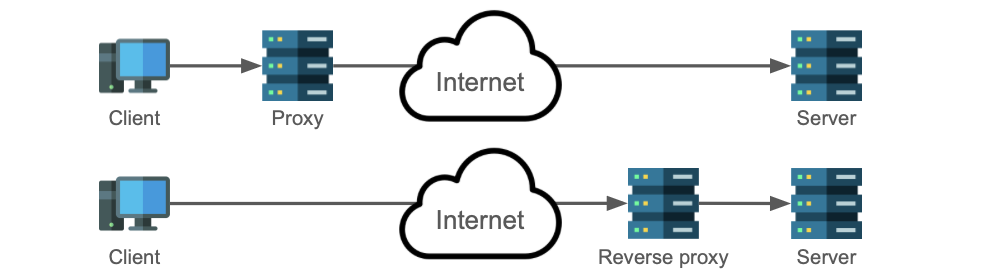
\includegraphics[width=0.8\textwidth]{proxy}
    \label{fig:LABEL}
\end{figure}
\begin{itemize}
	\item Direct proxies protect users when they access servers on the Internet
	\item Reverse proxies protect servers when accessed by users from the Internet
\end{itemize}

\section*{Web Proxies}

Goal: protect users surfing the web against threat by reducing attack surface. 
\begin{itemize}
	\item Analyse all data downloaded from the web
	\item Block access to dangerous sites
\end{itemize}

The browser must be configured to use the proxy

The firewall can be configured to only allow the proxy to access web sites, users cannot surf the net if they don't go through the proxy. 

\section*{Web Proxies for HTTPS}

\textbf{MitM Connections}

The proxy can be configured to intercept HTTPS traffic
Rather than forwarding the handshake, it pretends to be the server
\begin{itemize}
	\item To achieve this it must generate fake certificates
	\item The browser sees the fake certificate and wants to generate an error
	\item All browsers of the company must be configured to accept fake certificates from the proxy
\end{itemize}

\textbf{Passthrough}
By default, HTTPS traffic is encrypted from the client to the server

\begin{itemize}
	\item The proxy forwards the TLS handshake between the client and the server
	\item It just acts like a passthrough
	\item The client receives the original certificate
	\item The proxy only sees encrypted traffic: it cannot filter dangerous data
\end{itemize}

\textbf{Going Forward}

MitM proxying is getting more and more difficult due to technological advanced such as: 
\begin{itemize}
	\item HSTS for enforcing HTTPS
	\item certificate pinning for preventing certificate spoofing
	\item perfect forward secrecy of TLS 1.3 for using ephemeral keys to prevent later decryption 
\end{itemize}

\section*{Mail Gateways}

Mail gateways act both as proxy and reverse proxy: all outgoing mail is stored on the mail gateway before being forwarded to the internet

All incoming mail is intercepted by the gateway before being forwarded to the users' mailbox

Mail gateways typically offer:
\begin{itemize}
	\item antivirus protection
	\item incoming and outgoing spam protection
\end{itemize}

\section*{Web Application Firewall (WAF)}

A WAF is the typical example of reverse proxy with the goal of protecting a web server against malicious requests from the Internet

It analyses requests, and if it deems them safe, forwards them to the real server

WAFs typically offer the following protections: 
\begin{itemize}
	\item Block any request that seems to contain an attack (XSS, SQL, injection)
	\item Limit the number of requests to protect against DoS attacks (your site will still be unreachable, but at least your internal server still works)
	\item Block an IP address for a certain time after detection of an attack
	\item Authenticate users (to prohibit unauthenticated users from interacting

\end{itemize}

\textbf{Example:} modSecurity

modSecurity started as an Apache web server module and now protects diverse web servers and reverse proxies

There is a free open source set of rules (core rule set) with thousands of rules

SQL injection examples:
\begin{itemize}
	\item "@rx (?i)union.*?select.*?from"
	\item"@rx (?i:sleep\(\s*?\d*?\s*?\)|benchmark\(.*?\,.*?\))"
\end{itemize}
\section*{Intrusion Detection Systems}

An IDS inspects traffic for \textbf{\textit{all}} applications to detect potential detections:
\begin{itemize}
	\item Generates alerts if it thinks it saw an attack
	\item Called an Intrusion Prevention System (IPS) when it also blocks such traffic
\end{itemize}
Two technologies:
\begin{itemize}
	\item Signatures-based systems
	\item Anomaly-based systems
\end{itemize}

Possible issues:
\begin{itemize}
	\item False positives (too many alarms)
	\item False negatives (too many successful attacks)
\end{itemize}

\section*{Signature-based IDS}

Compares network traffic against signatures from a pattern database, like a WAF does for web traffic

Possible issues
\begin{itemize}
	\item Requires previous knowledge of an attack to create a signature (false negatives for new attacks)
	\item Matched signature does not always mean successful attack, e.g., signature for a Linux vulnerability in traffic of a Windows server (false positives)
\end{itemize}

Signature examples:
\begin{itemize}
	\item High number of failed login attempts
	\item URLs with extra long parameters (buffer overflows?)
	\item Exploiting a specific vulnerability: Cisco IOS invalid IKE fragment length memory corruption or exhaustion attempt
\end{itemize}

\section*{Signature-based IDS: Snort}

Snort sniffs traffic in front of your firewall to detect potential attacks. It sends alarms and/or updates to firewall, blocking the attacker. 

Large database of free rules maintained by community. Commercial database of additional rules. 

\section*{Anomaly-based Systems}

Goal: detect unknown attacks

The IDS create a \textbf{\textit{traffic profile}} during normal operation to calibrate. 

During monitoring, it looks for unusual packets, e.g., growth in port scans

\begin{itemize}
	\item Might not detect an SQL injection (extra characters in username)
	\item Might notice a 200MB transfer of password hashes from the database
\end{itemize}

Generates a lot of false positives and negatives (anomaly != attack)

\begin{itemize}
	\item Very hot applications for machine learning techniques!
\end{itemize}

\section*{Base Rate Fallacy}
Image a situation where:
\begin{itemize}
	\item the probability that a packet is part of an attack is 1 in 10,000
	\item the false positive rate of your IDS is 1\% for a single packet
	\item the false negative rate is 1\% for a single packet
	\item its 2am, you receive an alert from your IDS
\end{itemize}

The chance that that this is a true alarm is of 1\% only!! You should stay in bed. 
\vspace{0.5cm}

\begin{center}
  {\LARGE \textbf{Protecting a Workstation}}
\end{center}
\vspace{0.5cm}

Prevent exploitable bugs:
\begin{itemize}
	\item Ensure automatic update of the OS
	\item Ensure automatic update of the applications
\end{itemize}

Prevent known malware:
\begin{itemize}
	\item Install antivirus or use built-in ones (e.g., Windows Defender)
	\item Install applications from trusted sources (market of packet manager)
\end{itemize}

Prevent unknown malware:
\begin{itemize}
	\item Prohibit users from installing applications
	\item Restrict write access to directories that contain documents, not programs. 
\end{itemize}

\begin{tcolorbox}[
  colback=orange!15,     % background color
  colframe=black!50,    % border color
  boxrule=1pt,       % border thickness
  arc=3mm,             % rounded corners
  left=4mm, right=4mm, top=2mm, bottom=2mm % padding
  ]
AntiVirus is no longer as effective as campaigns are very short-lived
\end{tcolorbox}

\section*{Preventing Privilege Escalation}

Verify that all access rights are correctly set on programs and libraries. 

Typical issue: a program that is run by System is writable by any user, the attacker replaces the program by a malicious program and reboots the machine

Make sure that all program are regularly patched to fix any known vulnerabilities

Make sure that the hard disk is encrypted, if not, attackers can boot form USB (or remove the disk) and have full access rights to all files. 

\vspace{0.5cm}

\begin{center}
  {\LARGE \textbf{Protecting History: Logging}}
\end{center}
\vspace{0.5cm}
Keeping \textcolor{red}{audit trails} (aka logs) is an import part of network security. It helps identify security incidents, monitor policy violations, and non reputation control. Massive amount of logs being used by different services. 

Things that \textbf{you should never log}: 
\begin{itemize}
	\item Passwords!
	\item Religious, ideological, political or trade union-related views or activities
	\item Social security measures
	\item Administrative or criminal proceedings and sanctions
	\item etc...
\end{itemize}

\vspace{0.5cm}

\begin{center}
  {\LARGE \textbf{Protecting Data: Backups}}
\end{center}
\vspace{0.5cm}

\section*{Backup Recommendations}

Backup types: full, incremental (data that changed since last backup), differential (data that changes since last full backup)

3-2-1 rule:
\begin{itemize}
	\item 3 copies of the data
	\item On 2 different types of media (e.g, disk and tape)
	\item 1 stored off-site
\end{itemize}

\section*{Backup Content}

Backups are made differently depending on the type of data. Like virtual machines, databases, file storage all have different backup strategies. For instance databases have their own tools to backup and restore the content of their tables. 


\section*{Disaster Recovery Plan}

Making backups is not sufficient. Backups also need to be tested regularly through \textit{\textbf{restoration tests}}, i.e., to ensure we can recover data from backups

A Disaster Recovery Plan (DRP) records, in detail, how to rebuild a system in case of a major failure. 

\end{document}
